\documentclass[aspectratio=169]{beamer}
\usepackage[T1]{fontenc} \usepackage{lmodern} \usepackage[utf8]{inputenc}
\usepackage[english]{babel} \usepackage{booktabs}
\usepackage{graphicx,subcaption} \usepackage{amssymb,amsmath}
\graphicspath{{figures/}}
\usepackage[citestyle=authoryear,bibstyle=authoryear,backend=biber,url=false,doi=false,isbn=false]{biblatex} \bibliography{refs}
\usepackage{hyperref}

%------------------------------------------------

% https://hartwork.org/beamer-theme-matrix/
% http://www.cpt.univ-mrs.fr/~masson/latex/Beamer-appearance-cheat-sheet.pdf

% Sans-serif is easier to read. Keep for text.
% Math is nicer in serif, and easier to discriminate from text.
% But then it's inconsistent...
%\usefonttheme{serif}
\usefonttheme[onlymath]{serif}

\usetheme{Malmoe}
\setbeamertemplate{footline}[page number]
\setbeamertemplate{navigation symbols}{}

\definecolor{darkred}{rgb}{0.8,0,0}  % defined in beaver
\usecolortheme{beaver}
\setbeamercolor{structure}{fg=darkred,bg=white}
\setbeamercolor{block title}{fg=darkred,bg=white}

%------------------------------------------------

\newcommand{\HRule}{{\usebeamercolor[bg]{subsection in head/foot} \rule{\linewidth}{0.5mm}}}

%------------------------------------------------

\begin{document}

\begin{frame}[plain]
	%\titlepage
	\begin{center}

		\begin{minipage}{0.7\linewidth}
			\textsc{\large A Network Tour of Data Science}
		\end{minipage}
		\hfill
		\begin{minipage}{0.2\linewidth}
			\includegraphics[width=\linewidth]{logo_epfl}
		\end{minipage}
		\vspace{0.5cm}

		\HRule
		\vspace{0.55cm}
		{
			\usebeamercolor[fg]{frametitle}
			\textsc{\Large Practical Informations}\\
			%\textsc{\Large Lab Sessions}\\
			%\textsc{\Large Laboratories}\\
			\vspace{0.3cm}
		}
		\HRule
		\vspace{0.8cm}

		\hspace{0.3cm}
		\begin{minipage}[t]{0.35\linewidth}
			\footnotesize
			\textbf{Teachers} \\
			Pierre \textsc{Vandergheynst} \\
			Pascal \textsc{Frossard} \\
			Andreas \textsc{Loukas} \\
			Michaël \textsc{Defferrard} \\
			Volodymyr \textsc{Miz} \\
		\end{minipage}
		\begin{minipage}[t]{0.25\linewidth}
			\footnotesize
			\textbf{Assistants} \\
			Michaël \textsc{Defferrard} \\
			Volodymyr \textsc{Miz} \\
			Effrosyni \textsc{Simou} \\
			Eda \textsc{Bayram} \\
		\end{minipage}
		\begin{minipage}[t]{0.25\linewidth}
			\footnotesize
			Benjamin \textsc{Ricaud} \\
			Nicolas \textsc{Aspert} \\
			Clément \textsc{Vignac} \\
			Guillermo \textsc{Jimenez} \\
			Nikolaos \textsc{Karalias} \\
		\end{minipage}

		\vspace{0.4cm}
		{\footnotesize EPFL LTS2 \& LTS4 laboratories
		\hfill September 17, 2019}

	\end{center}
\end{frame}

%------------------------------------------------

\begin{frame}
	\frametitle{Team}
	\begin{figure}
		\centering
		\captionsetup{justification=centering}
		\begin{subfigure}[b]{0.14\linewidth}
			\includegraphics[width=\linewidth]{picture_pierre}
			\caption*{Pierre\\Vandergheynst}
		\end{subfigure}
		\hfill
		\begin{subfigure}[b]{0.14\linewidth}
			\includegraphics[width=\linewidth]{picture_pascal}
			\caption*{Pascal\\Frossard}
		\end{subfigure}
		\hfill
		\begin{subfigure}[b]{0.14\linewidth}
			\includegraphics[width=\linewidth]{picture_andreas}
			\caption*{Andreas\\Loukas}
		\end{subfigure}
		\hfill
		\begin{subfigure}[b]{0.14\linewidth}
			\includegraphics[width=\linewidth]{picture_michael}
			\caption*{Michaël\\Defferrard}
		\end{subfigure}
		\hfill
		\begin{subfigure}[b]{0.14\linewidth}
			\includegraphics[width=\linewidth]{picture_volodymyr}
			\caption*{Volodymyr\\Miz}
		\end{subfigure}
		\hfill
		\begin{subfigure}[b]{0.14\linewidth}
			\includegraphics[width=\linewidth]{picture_ersi}
			\caption*{Effrosyni\\Simou}
		\end{subfigure}
		\\
		\vspace{1em}
		\begin{subfigure}[b]{0.14\linewidth}
			\includegraphics[width=\linewidth]{picture_eda}
			\caption*{Eda\\Bayram}
		\end{subfigure}
		\hfill
		\begin{subfigure}[b]{0.14\linewidth}
			\includegraphics[width=\linewidth]{picture_benjamin}
			\caption*{Benjamin\\Ricaud}
		\end{subfigure}
		\hfill
		\begin{subfigure}[b]{0.14\linewidth}
			\includegraphics[width=\linewidth]{picture_nicolas}
			\caption*{Nicolas\\Aspert}
		\end{subfigure}
		\hfill
		\begin{subfigure}[b]{0.14\linewidth}
			\includegraphics[width=\linewidth]{picture_clement}
			\caption*{Clément\\Vignac}
		\end{subfigure}
		\hfill
		\begin{subfigure}[b]{0.14\linewidth}
			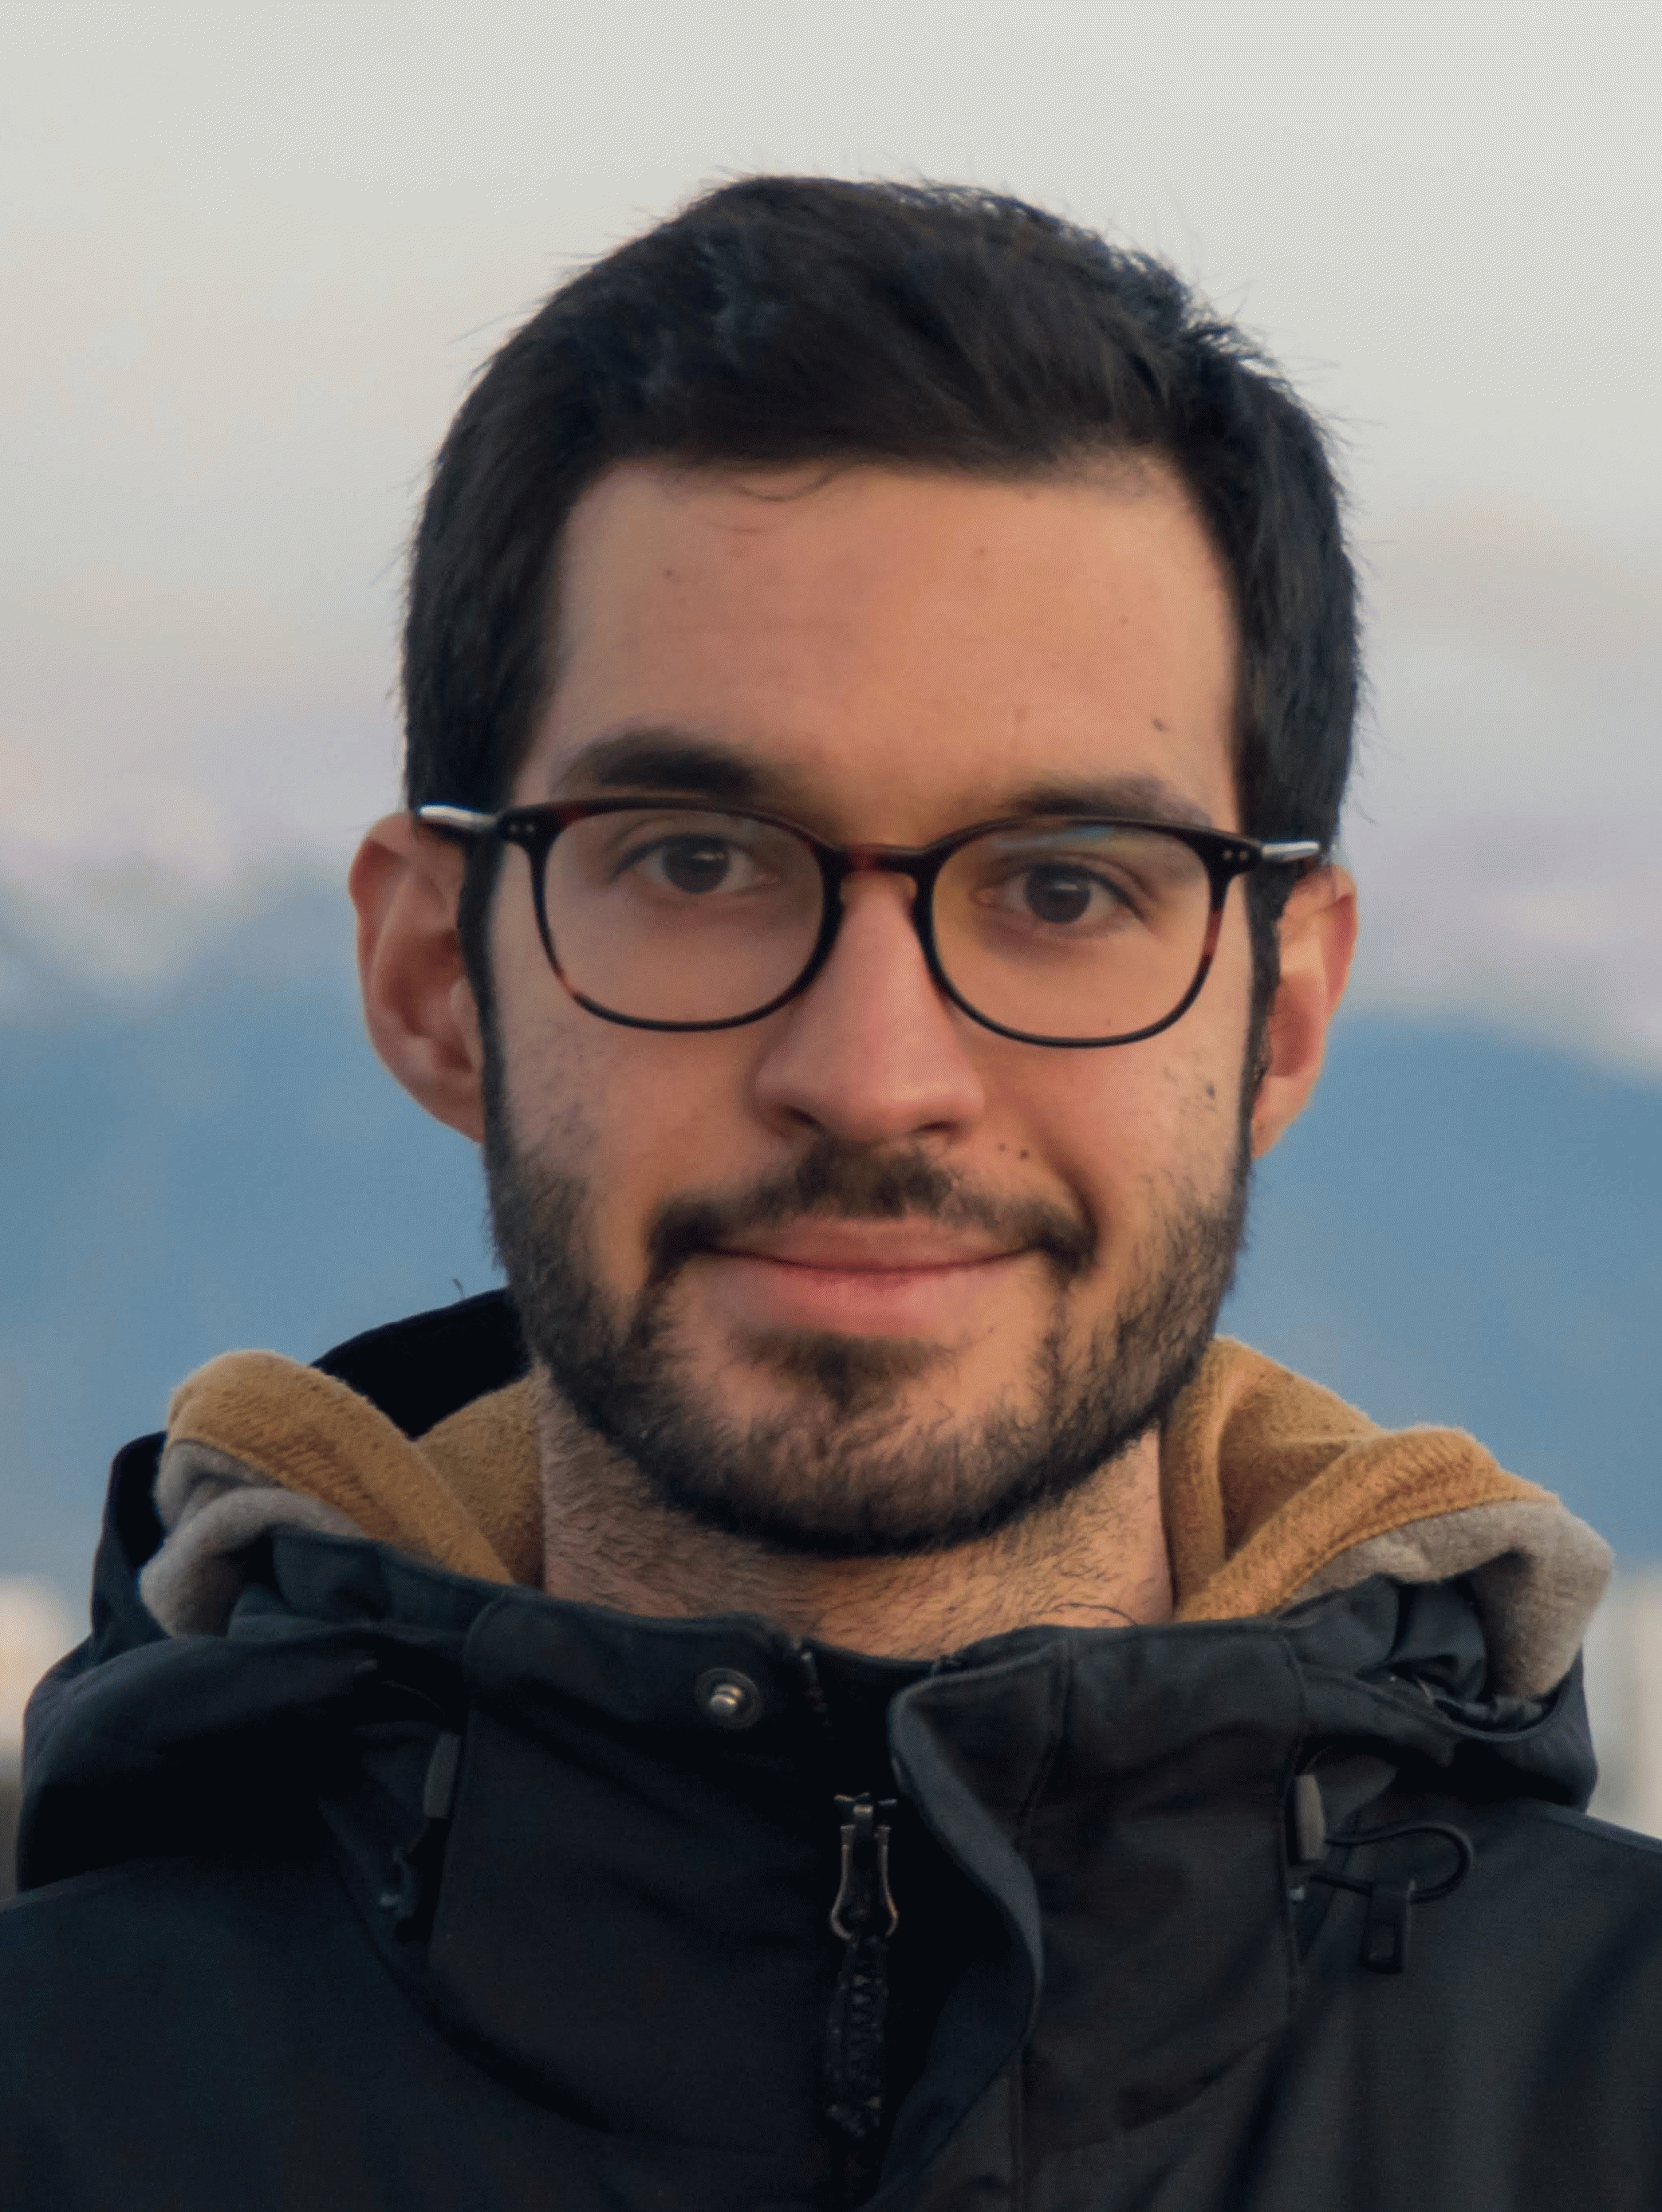
\includegraphics[width=\linewidth]{picture_guillermo}
			\caption*{Guillermo\\Jimenez}
		\end{subfigure}
		\hfill
		\begin{subfigure}[b]{0.14\linewidth}
			\includegraphics[width=\linewidth]{picture_nikos}
			\caption*{Nikolaos\\Karalias}
		\end{subfigure}
	\end{figure}
\end{frame}

%------------------------------------------------

\begin{frame}
	\frametitle{Enrollment}
	% Poll: from which section are you from.
	\centering
	\includegraphics[width=0.9\linewidth]{enrollment}
\end{frame}

%------------------------------------------------

\begin{frame}
	\frametitle{Content: \textbf{A Network Tour} of Data Science}
	% First networks alone. Then data on networks.
	\begin{minipage}{0.41\linewidth}
		\begin{enumerate}
			\item Network Science
			\vspace{2em}
			\item Spectral Graph Theory
			\vspace{2em}
			\item Graph Signal Processing
			\vspace{2em}
			\item Machine Learning with Graphs
		\end{enumerate}
	\end{minipage}
	\hfill
	\begin{minipage}{0.57\linewidth}
		\includegraphics[width=\linewidth]{fma_illustration}
	\end{minipage}
\end{frame}

%------------------------------------------------

\begin{frame}
	\frametitle{Content: A Network Tour of \textbf{Data Science}}
	\begin{figure}
		\includegraphics[height=0.85\textheight]{data_scientist}
	\end{figure}
\end{frame}

%------------------------------------------------

\begin{frame}
	\frametitle{Organization}
	\begin{block}{Theory \& practice}
	\begin{description}
		\item[Lectures] theory and tools to deal with networks and network data
		\item[Lab sessions] application of the tools to real-world data
	\end{description}
	\end{block}
	\vfill
	Sessions on Tuesdays (10:15 to 12:00, CE2) and Wednesdays (10:15 to 12:00, CO2)
	\vfill
	\begin{block}{Course support}
	\begin{itemize}
		\item your notes
		\item lecture slides (available on Moodle)
		\item research papers and textbooks referenced in the slides
	\end{itemize}
	\end{block}
\end{frame}

%------------------------------------------------

\begin{frame}
	\frametitle{Schedule}
	\framesubtitle{(tentative, updated on Moodle)}
	\begin{figure}
		\includegraphics[width=\linewidth,trim={0 8.2cm 0 0.8cm},clip]{ntds2019_schedule_v4}
	\end{figure}
\end{frame}

%------------------------------------------------

\begin{frame}
	\frametitle{Schedule}
	\framesubtitle{(tentative, updated on Moodle)}
	\begin{figure}
		\includegraphics[width=\linewidth,trim={0 0 0 8.6cm},clip]{ntds2019_schedule_v4}
	\end{figure}
\end{frame}

%------------------------------------------------

\begin{frame}
	\frametitle{Deadlines}
	\framesubtitle{(tentative, announced on Moodle)}
	\begin{description}
		\item[Oct 1] form groups of four %and choose a project
		\vfill
		\item[Oct 15] handle assignment 1 (network properties \& models)
		\vfill
		\item[Nov 19] handle assignment 2 (spectral, GSP, GNN)
		\vfill
		\item[Dec 4] handle project summary for peer-review
		\vfill
		\item[Dec 10] handle peer-review report
		\vfill
		\item[Jan 10] handle project report and github repository
		\vfill
		\item[Jan 21] project presentations
	\end{description}
\end{frame}

%------------------------------------------------

\begin{frame}
	\frametitle{Practical sessions}
	\begin{center}
		Apply the material learned in class in a Data Science context.
	\end{center}
	\vfill
	During the labs, we will:
	\begin{itemize}
		\item Demo tools, e.g., how to manipulate a graph in Python.
		\item Explain the assignments and give directions.
		\item Answer questions about the assignments and project.
	\end{itemize}
	\vfill
	We expect you to:
	\begin{itemize}
		\item Bring your laptop.
		\item Work outside the hours on the assignments and project.
	\end{itemize}
\end{frame}

%------------------------------------------------

\begin{frame}
	\frametitle{Tools: Python scientific stack}
	\framesubtitle{To be installed with \href{https://conda.io}{conda}.}
	% Poll the students.
	% Raise your hand if you programmed in Python. Who didn't? git?
	\begin{minipage}{0.45\linewidth}
	\begin{itemize}
		\item \href{https://git-scm.com}{git}: version control system
		\vspace{0.7em}
		\item \href{https://www.python.org}{Python}: programming language
		\vspace{0.7em}
		\item \href{https://jupyter.org}{Jupyter}: interactive computing
		\vspace{0.7em}
		\item \href{http://www.numpy.org}{NumPy}: $n$-dimensional arrays
		\vspace{0.7em}
		\item \href{https://www.scipy.org/scipylib}{SciPy}: scientific computing
		\vspace{0.7em}
		\item \href{https://matplotlib.org}{matplotlib}: visualization
	\end{itemize}
	\end{minipage}
	\hfill
	\begin{minipage}{0.45\linewidth}
	\begin{itemize}
		\item \href{https://pandas.pydata.org}{pandas}: data analysis
		\vspace{0.7em}
		\item \href{https://networkx.github.io}{NetworkX}: network science
		\vspace{0.7em}
		\item \href{https://graph-tool.skewed.de}{graph-tool}: network science
		\vspace{0.7em}
		\item \href{https://pytorch.org}{gephi}: graph visualization
		\vspace{0.7em}
		\item \href{https://github.com/epfl-lts2/pygsp}{PyGSP}: graph signal processing
		\vspace{0.7em}
		\item \href{https://pytorch.org}{PyTorch}: deep learning
	\end{itemize}
	\end{minipage}
\end{frame}

%------------------------------------------------

\begin{frame}
	\frametitle{Evaluation}
	Joint evaluation of theoretical and practical skills through assignments and a project.
	\vfill
	Two parts:
	\begin{enumerate}
		\item Guided with two assignments that follow the lectures.
		\item Open ended project.
	\end{enumerate}
	\vfill
	\begin{block}{Grading}
	\begin{description}
		\item[assignments] 50\% for acquiring the course material in a structured way
		\item[peer-review] 10\% for giving critical feedback
		\item[project] 40\% for being creative and able to understand data, i.e., Data Science
	\end{description}
	\end{block}
\end{frame}

%------------------------------------------------

\begin{frame}
	\frametitle{Assignments}
	\begin{enumerate}
		\item Template notebook with instructions given on GitHub.
		\item Multiple weeks to complete.
		\item Lab sessions to ask questions.
		\item Completed notebook to be handled on Moodle.
		\item Solutions posted on GitHub.
		\item Grades given on Moodle.
	\end{enumerate}
	\vfill
	Topics that follow the lectures, with a Data Science taint:
	\begin{enumerate}
		\item Network properties \& models
		\item Spectral Graph Theory, Graph Signal Processing, Graph Neural Networks
	\end{enumerate}
\end{frame}

%------------------------------------------------

\begin{frame}
	\frametitle{Project}
	\framesubtitle{More information later in the semester.}
	\begin{center}
		Tell us a data story based on the course material!
	\end{center}
	\vfill
	\begin{enumerate}
		\item Form teams of four and choose a project.
		\vfill
		\item Write a summary and get critical feedbacks from peers. %Improve based on feedbacks.
		\vfill
		\item Handle a report and a git repository with code.
		\vfill
		\item Impress us in a presentation!
	\end{enumerate}
\end{frame}


%------------------------------------------------

\begin{frame}
	\frametitle{Data science process}
	\begin{figure}
		\includegraphics[height=0.85\textheight]{data_science_process}
	\end{figure}
\end{frame}

%------------------------------------------------

\begin{frame}
	\frametitle{Some projects from 2018}
	\framesubtitle{more at \url{https://github.com/mdeff/ntds_2018}}
	\begin{figure}
		\includegraphics[width=0.87\linewidth]{projects_2018}
	\end{figure}
\end{frame}

%------------------------------------------------

\begin{frame}
	\frametitle{Online}
	\begin{block}{Moodle, \url{https://moodle.epfl.ch/course/view.php?id=15299}}
	\begin{minipage}{0.25\linewidth}
	\begin{itemize}
		\item slides
		\item grades
	\end{itemize}
	\end{minipage}
	\begin{minipage}{0.45\linewidth}
	\begin{itemize}
		\item official announcements
		\item discussion forum
	\end{itemize}
	\end{minipage}
	\end{block}
	\vspace{1em}
	\begin{block}{GitHub, \url{https://github.com/mdeff/ntds_2019}}
	\begin{minipage}{0.25\linewidth}
	\begin{itemize}
		\item assignments
		\item projects
	\end{itemize}
	\end{minipage}
	\begin{minipage}{0.45\linewidth}
	\begin{itemize}
		\item installation instructions
		\item tutorials
	\end{itemize}
	\end{minipage}
	\end{block}
	\vfill
	\begin{center}
		\Huge Questions?
	\end{center}
\end{frame}

%------------------------------------------------

\end{document}
